 \section{Architektura}
 Cílem této práce je vytvoření programu, který bude schopen detekovat anomální provoz v IoT sítích. 
 Vzhledem k hardwarovým omezením, které můžou na IoT branách nastat, je architektura navržena tak, aby
 měla co nejmenší nároky na dostupné prostředky. Schéma nasazení detekčního systému se nachází
 na obrázku \ref{obr.deploy-arch}
 
 \begin{figure}[ht]
   \begin{center}
   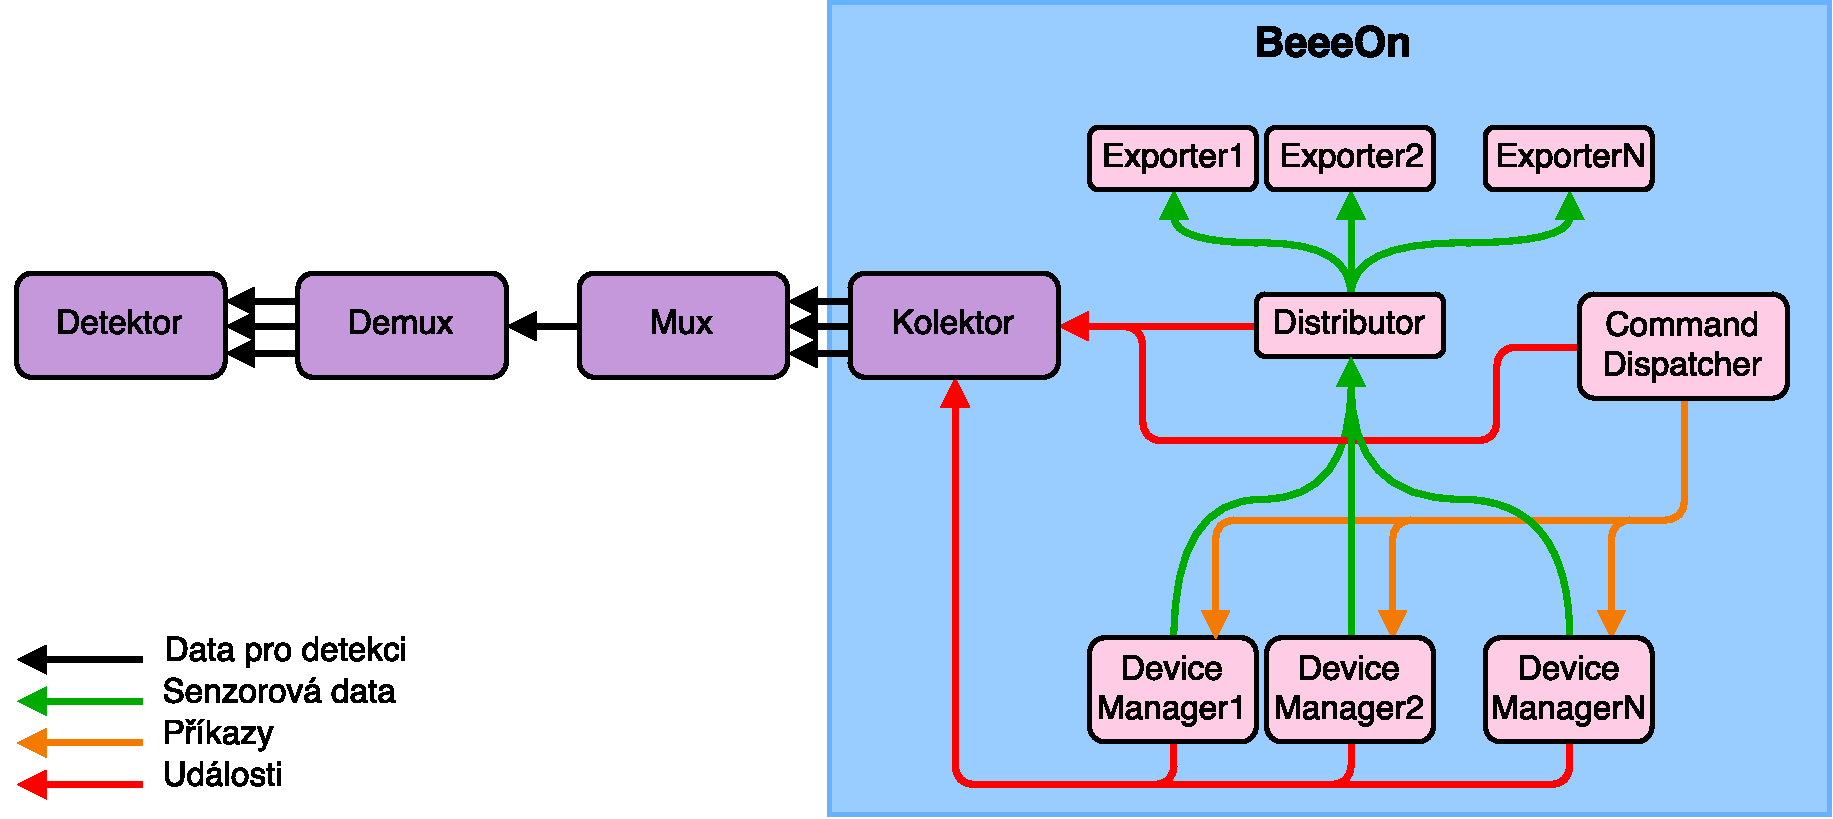
\includegraphics[scale=0.41]{pictures/deploy-arch}
   \caption{Architektura detekčního systému}
   \label{obr.deploy-arch}
   \end{center}
   \end{figure}
 
 Implementace BeeeOn brány obsahuje pro zpracování senzorových dat následující komponenty:
 \begin{itemize}
  \item \textbf{DeviceManager}:
    komponenta definovaná pro každý senzorový protokol, která implementuje veškerou komunikaci
    a zpracování dat
    
  \item \textbf{Distributor}:  
  přijímá data od \textit{DeviceManageru}, která nasledně předává příslušnému \textit{Exporteru}
  
  \item \textbf{Exporter}:
  implementuje protokol, kterým jsou data odesílány z brány
  
  \item \textbf{CommandDispatcher}:  
  komponenta, která přijímá uživatelské příkazy a distribuuje je cílovým komponentám
  
 \end{itemize}
 
 Každá z komponent v BeeeOn bráně navíc využívá návrhový vzor Observer, pomocí kterého jsou
 definovany události poskytující informace o každé komponentě. 
 Tímto způsobem bude vytvořený kolektor zíkávat data o provozu, která
 převede do fomátu UniRec (Unified Record) a pomocí systému NEMEA je odešle k analýze.
 
 Exportované informace o provozu bude přijímat detektor, který následně provede jejich zpracování a 
 vyhodnocení stavu. Všechny vytvořené komponety vytvořené pro detekci budou používat rozhraní 
 NEMEA. Díky tomu bude možné komponenty flexibilně provozovat na jednom nebo více různých zařízeních.
 Oddělené nasazení je důležité zejména pro brány s omezenými prostředky, které mohou provádět 
 pouze export dat a o vyhodnocení se bude starat odlišné zařízení s dostatečným výkonem. V případě 
 provozování více bran lze brány používat jako exportéry a veškerá získaná data zpracovávat 
 centrálně. 
 
 Kolektor pro každou událost vytvoří samostnatné výstupní rozhraní. Protože událostí může být 
 velké množství, tak bude vytvořen modul \textit{Mux}, který všechny výstupní rozhraní spojí do jednoho. 
 Pro zpětné rozdělení na jednotlivá rozhraní budou dloužit modul \textit{Demux}. Tyto moduly budou velmi užitečné
 zejména v případě kdy kolektor a detektor budou na rozdílných síťových prvcích, protože údaje 
 o provozu budou přenášeny přes počítačovou síť a bude vyžadováno zabezpeční všech odchozích
 rozhraní. S využítím \textit{Mux} a \textit{Demux} modulů bude stačit zabezpečit pouze jedno sjednocené rozhraní. 
 
 Výhodou návrhu řešení je flexibilita a modularita. Každá komponenta vždy samostatně pokrývá pouze jednu
 část detekčního systému a se díky NEMEA se každá z nich může nacházet na různých síťových prvcích. Zároveň
 v případě potřeby lze vytvořit další moduly, které budou rozšiřovat stávající funcionalitu.
 Podrobnější popis návrhu nově vytvořených komponent detekčního systému se nachází v následujících kapitolách.
 
 \section{Kolektor}
 Úkolem kolektoru bude sběr dostupných dat a jejich odeslání k následné analýze. Informace o 
 provozu budou sbírány z jednotlivých komponent BeeeOn brány, které jsou zpřístupňovány pomocí 
 návrhového vzoru Observer. Z tohoto důvodu bude kolektor vždy přímou součástí BeeOn brány. 
 Návrh struktury kolektoru je na obrázku 
 
 \begin{figure}[ht]
   \begin{center}
   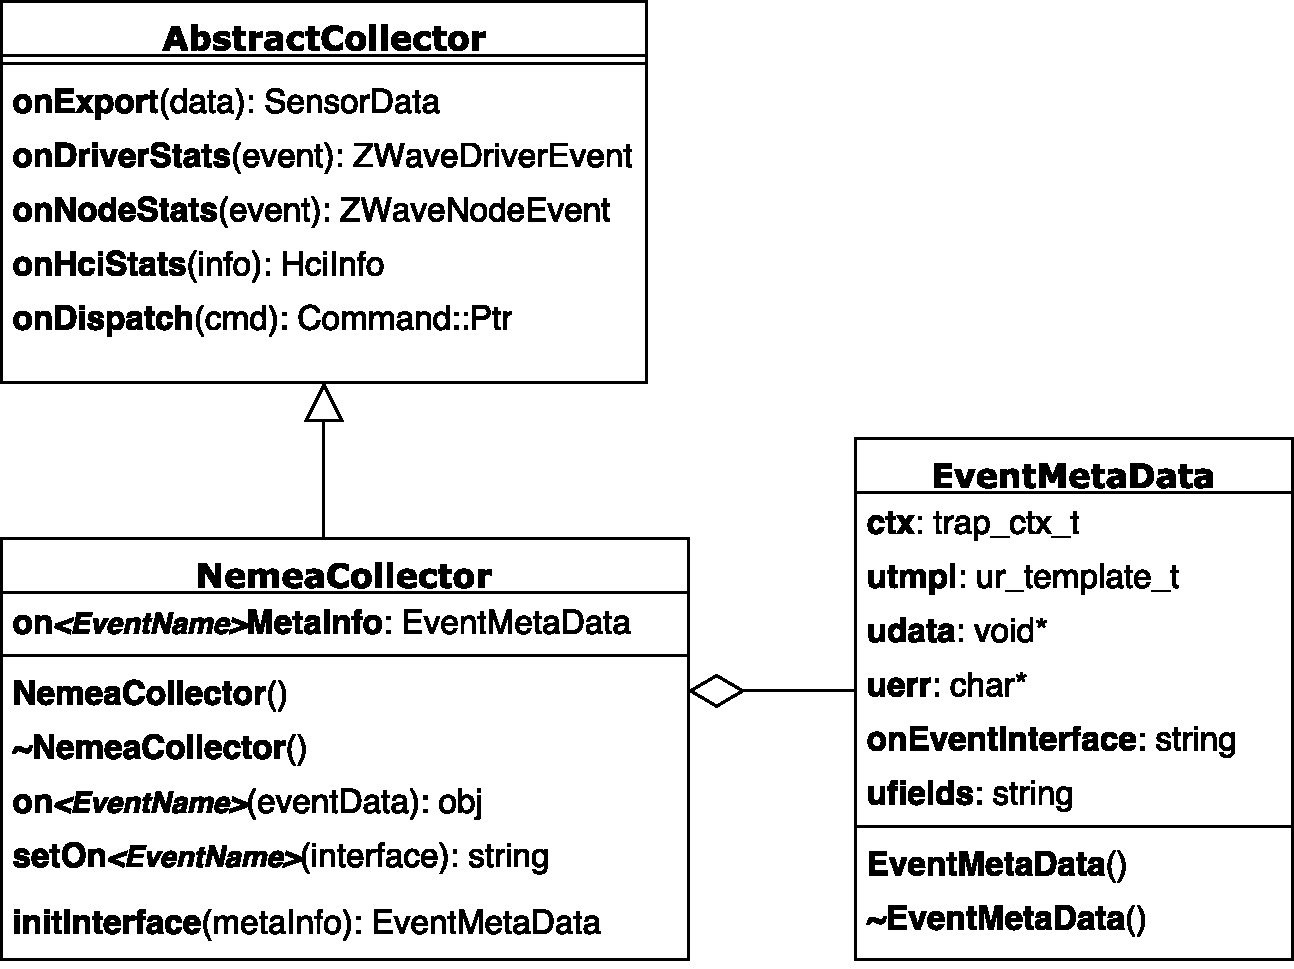
\includegraphics[scale=0.5]{pictures/modelTrid}
   \caption{Návrh kolektoru provozních dat}
   \label{obr.modelTrid}
   \end{center}
   \end{figure}
 
 obecné povídání o kolektoru - je vždy součástí brány
 návrh method a tříd v bráně
    
 \section{Detektor}
  časové řady
  univerzální návrh který umožňuje použití více nebo jen jednoho detektoru
  Sytaxe konfiguračního souboru - klíč hodnoty
  návrh metod a tříd 
  
 \section{Multiplexor a demultiplexor}
 
 \section{Scénáře útoků}
